%%%% Proceedings format for most of ACM conferences (with the exceptions listed below) and all ICPS volumes.
\documentclass[sigconf]{acmart}
\usepackage{algorithm}
\usepackage[export]{adjustbox}
\usepackage[noend]{algpseudocode}
\usepackage{todonotes}
\usepackage{xspace}
\usepackage{listings}
%\usepackage{subcaption}
\usepackage{paralist}

\newcommand{\mpifunc}[1]{\lstinline"MPI_#1"\xspace}
\newcommand{\prrte}[0]{\textsc{PRRTE}\xspace}
\newcommand{\pmix}[0]{\textsc{PMIx}\xspace}
\newcommand{\orte}[0]{\textsc{Open~RTE}\xspace}
\newcommand{\ompi}[0]{\textsc{Open~MPI}\xspace}
\newcommand{\ulfm}[0]{\textsc{ULFM}\xspace}
\newcommand{\mpi}[0]{\textsc{MPI}\xspace}
\newcommand{\oshmem}[0]{\textsc{OpenSHMEM}\xspace}
\newcommand{\ourwork}[0]{\textsc{RDaemon}\ensuremath{^\#}\xspace}

\newcommand{\imb}[0]{\textsc{IMB}\xspace}

%%%% As of March 2017, [siggraph] is no longer used. Please use sigconf (above) for SIGGRAPH conferences.

%%%% Proceedings format for SIGPLAN conferences
% \documentclass[sigplan, anonymous, review]{acmart}

%%%% Proceedings format for SIGCHI conferences
% \documentclass[sigchi, review]{acmart}

%%%% To use the SIGCHI extended abstract template, please visit
% https://www.overleaf.com/read/zzzfqvkmrfzn

%
% defining the \BibTeX command - from Oren Patashnik's original BibTeX documentation.
\def\BibTeX{{\rm B\kern-.05em{\sc i\kern-.025em b}\kern-.08emT\kern-.1667em\lower.7ex\hbox{E}\kern-.125emX}}

% Rights management information.
% This information is sent to you when you complete the rights form.
% These commands have SAMPLE values in them; it is your responsibility as an author to replace
% the commands and values with those provided to you when you complete the rights form.
%
% These commands are for a PROCEEDINGS abstract or paper.
\copyrightyear{2019}
\acmYear{2019}
\setcopyright{licensedusgovmixed}
\acmConference[EuroMPI '19]{EuroMPI '19: ACM International Conference Proceeding Series}{September 11th-13th, 2019}{Zurich, Switzerland}
\acmPrice{15.00}
\acmDOI{10.1145/1122445.1122456}
\acmISBN{978-1-4503-9999-9/18/06}

%
% These commands are for a JOURNAL article.
%\setcopyright{acmcopyright}
%\acmJournal{TOG}
%\acmYear{2018}\acmVolume{37}\acmNumber{4}\acmArticle{111}\acmMonth{8}
%\acmDOI{10.1145/1122445.1122456}

%
% Submission ID.
% Use this when submitting an article to a sponsored event. You'll receive a unique submission ID from the organizers
% of the event, and this ID should be used as the parameter to this command.
%\acmSubmissionID{123-A56-BU3}

%
% The majority of ACM publications use numbered citations and references. If you are preparing content for an event
% sponsored by ACM SIGGRAPH, you must use the "author year" style of citations and references. Uncommenting
% the next command will enable that style.
%\citestyle{acmauthoryear}

%
% end of the preamble, start of the body of the document source.
\begin{document}

%
% The "title" command has an optional parameter, allowing the author to define a "short title" to be used in page headers.
\title{Runtime Level Failure Detection and Propagation in HPC Systems}

%
% The "author" command and its associated commands are used to define the authors and their affiliations.
% Of note is the shared affiliation of the first two authors, and the "authornote" and "authornotemark" commands
% used to denote shared contribution to the research.
\author{Dong Zhong}
%\orcid{1234-5678-9012}}
%\email{dzhong@vols.utk.edu}
\orcid{0000-0002-7651-2059}
\affiliation{%
  \institution{The University of Tennessee}
  \streetaddress{1122 Volunteer Blvd}
  \city{Knoxville}
  \state{TN}
  \postcode{37996}
  \country{USA}
}
\author{Aurelien Bouteiller}
\orcid{0000-0001-5108-509X}
%\email{bouteill@icl.utk.edu}
\affiliation{%
  \institution{The University of Tennessee}
  \streetaddress{1122 Volunteer Blvd}
  \city{Knoxville}
  \state{TN}
  \postcode{37996}
  \country{USA}
}
\author{Xi Luo}
%\orcid{1234-5678-9012}}
%\email{xluo12@vols.utk.edu}
\affiliation{%
  \institution{The University of Tennessee}
  \streetaddress{1122 Volunteer Blvd}
  \city{Knoxville}
  \state{TN}
  \postcode{37996}
  \country{USA}
}
\author{George Bosilca}
\orcid{0000-0003-2411-8495}
%\email{bosilca@icl.utk.edu}
\affiliation{%
  \institution{The University of Tennessee}
  \streetaddress{1122 Volunteer Blvd}
  \city{Knoxville}
  \state{TN}
  \postcode{37996}
  \country{USA}
}

%\author{Jack J. Dongarra}
%\orcid{0000-0003-3247-1782}
%\email{dongarra@icl.utk.edu}
%\affiliation{%
%  \institution{The University of Tennessee}
%  \streetaddress{1122 Volunteer Blvd}
%  \city{Knoxville}
%  \state{TN}
%  \postcode{37996}
%  \country{USA}
%}
%
% By default, the full list of authors will be used in the page headers. Often, this list is too long, and will overlap
% other information printed in the page headers. This command allows the author to define a more concise list
% of authors' names for this purpose.
%\renewcommand{\shortauthors}{Zhong, Bouteiller, et al.}

%
% The abstract is a short summary of the work to be presented in the article.
\begin{abstract}
As the scale of high-performance computing (HPC) systems continues to grow, mean-time-to-failure (MTTF) of these HPC systems is negatively impacted and tends to decrease. In order to efficiently run long computing jobs on these systems, handling system failures becomes a prime challenge. We present here the design and implementation of an efficient runtime-level failure detection and propagation strategy targeting large-scale, dynamic systems that is able to detect both node and process failures. Multiple overlapping topologies are used to optimize the detection and propagation, minimizing the incurred overheads and guaranteeing the scalability of the entire framework.
% A ring topology is maintained by allowing one node sending and receiving periodically heartbeat to/from another node to detect a node failure(observing another single node). For process failure each host node (is in charge of monitoring) monitors its children processes. The propagation use a reliable broadcast method over a binomial graph(an arbitrary communication topology) to distribute error message to applications, guarantees a logarithmic propagate time.
The resulting framework has been implemented in the context of a system-level runtime for parallel environments, \pmix Reference RunTime Environment (\prrte), providing efficient and scalable capabilities of fault management to a large range of programming and execution paradigms.
% the algorithms and strategies proposed have a larger scope of most distributed programming environment.
This result is supported by an experimental evaluation of the resulting software stack on different machines.
\end{abstract}

%
% The code below is generated by the tool at http://dl.acm.org/ccs.cfm.
% Please copy and paste the code instead of the example below.
%
\begin{CCSXML}
<ccs2012>
<concept>
<concept_id>10010520.10010521.10010537</concept_id>
<concept_desc>Computer systems organization~Distributed architectures</concept_desc>
<concept_significance>500</concept_significance>
</concept>
<concept>
<concept_id>10010520.10010521.10010542.10010546</concept_id>
<concept_desc>Computer systems organization~Heterogeneous (hybrid) systems</concept_desc>
<concept_significance>300</concept_significance>
</concept>
<concept>
<concept_id>10010520.10010575.10010577</concept_id>
<concept_desc>Computer systems organization~Reliability</concept_desc>
<concept_significance>300</concept_significance>
</concept>
<concept>
<concept_id>10010520.10010575.10011743</concept_id>
<concept_desc>Computer systems organization~Fault-tolerant network topologies</concept_desc>
<concept_significance>300</concept_significance>
</concept>
<concept>
<concept_id>10011007.10010940.10011003.10011005</concept_id>
<concept_desc>Software and its engineering~Software fault tolerance</concept_desc>
<concept_significance>300</concept_significance>
</concept>
<concept>
<concept_id>10011007.10011006.10011041.10011048</concept_id>
<concept_desc>Software and its engineering~Runtime environments</concept_desc>
<concept_significance>300</concept_significance>
</concept>
</ccs2012>
\end{CCSXML}

\ccsdesc[500]{Computer systems organization~Distributed architectures}
\ccsdesc[300]{Computer systems organization~Heterogeneous (hybrid) systems}
\ccsdesc[300]{Computer systems organization~Reliability}
\ccsdesc[300]{Computer systems organization~Fault-tolerant network topologies}
\ccsdesc[300]{Software and its engineering~Software fault tolerance}
\ccsdesc[300]{Software and its engineering~Runtime environments}

%
% Keywords. The author(s) should pick words that accurately describe the work being
% presented. Separate the keywords with commas.
\keywords{fault tolerance, failure detection, reliable broadcast, message propagation, HPC runtime system}

%
% This command processes the author and affiliation and title information and builds
% the first part of the formatted document.
\maketitle

\section{Introduction}\label{sec:intro}

The complexity and vastness of the questions posed by modern science has
fueled the emergence of an era where exploring the boundaries of matter, life,
and human knowledge requires large instruments, either to perform the
experiments, collect the observation, and in the
case of high-performance computing (HPC), perform the compute-intensive
analysis of scientific data. As the march of science continues, small and
easy problems have already been solved, and significant advances increasingly
require tackling finer-grain, more accurate problems, which entails larger compute workloads, fueling an unending need for larger
HPC systems.

In turn, facing hard limits on power consumption and chip frequency,
HPC architects have been forced to embrace massive parallelism as well as
a deeper and more complex component hierarchy (e.g., non-uniform memory architectures,
GPU-accelerated nodes) to continue the growth in compute capabilities.
This has stressed the traditional HPC software infrastructure in different
ways, but it notably put to prominence two different issues that had been
largely disregarded in the last two decades: fault tolerance and novel programming
models.

The Message Passing Interface (MPI) has been instrumental in
permitting the efficient programming of massively parallel systems, scaling
along from early systems with tens of processors to current systems routinely
encompassing hundreds of thousands of cores. As failures become more
common on large and complex systems, The \mpi standard is in the process of
evolving to integrate fault tolerance capabilities, as proposed in the
User-Level Failure Mitigation (\ulfm) specification draft~\cite{Bland2013}, or
various efforts to integrate tightly checkpoint-restart with \mpi~\cite{reinit18}.
The second source of stress comes from programming systems that are inherently
hierarchical. This has brought forth a renaissance in the field of
programming models, leading to a variety of contenders challenging the
hegemony of \mpi as the sole method of harnessing the power of parallel systems.
Naturally, these alternatives to \mpi also have to handle fault tolerance~\cite{7161563, doi:10.1177/1094342016669416, shmem-ft15, 10.1007/978-3-319-50995-2_5, X10-ft16}.
In addition, the convergence
between big data infrastructure and the HPC infrastructure, as well as
the emergence of machine learning as a massive consumer of compute
capabilities, is gathering around HPC systems new communities that
have long-held expectations that the infrastructure provide resilience as a core feature~\cite{hadoop-ft}.

A feature that's commonly needed by these communities with a vested
interest in fault tolerance is the capability to efficiently, quickly and
accurately detect and report failures, so that they can manifest as
error codes from the programming interface, or trigger implicit recovery
actions. In prior works~\cite{George16}, we have designed a tailor-made
failure detector for \mpi that deploys finely tuned optimizations to
improve its performance. These optimizations are unfortunately strongly
tied to the \mpi internal infrastructure. For example, a key parameter to
the performance of that detector is the
access to low-level remote memory access routines, which may not be typically
available in a less \mpi-centric context. Similar concepts could be
applied to other HPC networking interfaces (e.g., \oshmem), but at
the expense of a major infrastructure rewrite for each and every one of
them. In this paper, we test the hypothesis that a fully dedicated \mpi
solution is not necessary to achieve great accuracy and performance, and
that a generic failure detection solution, provided by an external runtime
entity that does not have access to the \mpi context and communication conduits
can deliver a similar level of service. In order to test that hypothesis,
and further, to define how a generic one can provide the solution, we designed
a multi-level failure detection algorithm, called \ourwork, which operates
within the runtime infrastructure to monitor both node and process
failures. We implemented that algorithm as a component in the \pmix~\cite{CASTAIN18} runtime reference implementation (\prrte), which is a fully fledged runtime that is
used in production to deploy, monitor and
serve multiple HPC networking stack clients.
%like \ompi, or the reference \oshmem implementation. 
We then compare this generic
failure detection service with the fully dedicated \mpi detector from
\ulfm \ompi on one hand, and with the Scalable Weakly-Consistent Infection-style Membership (SWIM) protocol on the other hand, the latter standing
as a state-of-the-art detector for unstructured peer-to-peer systems. Henceforth
we highlight that there is a performance trade-off in generality, but
satisfactory level of performance can be achieved in a portable and reusable
component that can satisfy the needs of a variety of HPC networking systems.

The rest of this paper is organized as follows. Section~\ref{sec:motivation}
motivates our study and provides use cases and background on the \mpi specific
failure detector implementation in \ulfm. Section~\ref{sec:related} presents
related work on failure detectors followed by Section~\ref{sec:design} where we
describe the algorithm and implementation details of our generic failure
detector. Section~\ref{sec:experiments} describes the performance and accuracy
comparison between three different failure detectors providing a distinct
trade-off on the general to specific scale.

\section{Motivation and Background}\label{sec:motivation}
\todo{this is very rough, needs to be refocused in terms of motivating use cases}

Many projects have proposed fault management techniques either automatic or driven by the application or by a intermediary library, and most of these approaches rely on their own infrastructure to detect, propagate and react to failures. This leads to a very large number of partial solutions hardly maintained where no portable and efficient support to build resilient applications or programming models exists. This lack of reliable software infrastructure also make difficult to fairly compare existing or proposed solutions not only in terms of potential capabilities but in terms of performance. We believe it is critical to level the field and provide a resilient, efficient and portable fault detector and propagator, integrated into one of the most widely used parallel execution runtime, that allow other libraries and programming models to more construct and provide resilient capabilities at any scale. Here are some examples of potential users of such a resilient framework that we are actively pursuing.

\textbf{\ulfm:} \ourwork supports the functionality in \ulfm of revocation and correction of a broken communicator after node failure. For \ulfm the global communicator could be reconfigured after process failure detection, the failed processes are excluded from the global communicator using the \mpifunc{Comm_shrink} and are re-spawned using the \mpi function \mpifunc{Comm_spawn}, but the job will be aborted with node failure. However, using \ourwork instead of \ompi runtime the job doesn't need to be terminated after node failure. And with \ourwork's notification \mpi application can get the consensus knowledge of failure, then application can use the recovery functions (Shrink, Respawn) provided by \ulfm to build new communicator without the failed processes but with those newly spawned ones.
\todo{add SHMEM, REINIT; thinking about moving this part as 2. Motivation}

\textbf{\oshmem:} fault tolerance model is based on check-point and restart, that suits to the one-sided nature of PGAS programming model while leveraging features very specific to \oshmem. \ourwork failure detection and propagation attributes provide the flexibility to application developers to modulate the frequency and placement within the application where the checkpoint may be introduced. Also the notification provides the trigger for recovery.

\textbf{EREINIT:} \todo{this reads as related work} a global-restart failure recovery model by allowing a fast re-initialization of \mpi. This work is a co-design between MVAPICH and Slurm resource manager to add process and node failure detection and propagation features. The detection is using Slurm's health check mechanism by sending ping messages to nodes, propagation is implemented in a manner of forcing the controller to individually send the notification to children of the failed nodes. However this work is highly depends on one particular resource manager Slurm, also it use a inefficient propagation method. \ourwork work can exceed the bottleneck of EREINIT to run on machines with different resource managers(Slurm, PBS, LSF, TORQUE, etc). Also with our efficient propagation algorithm the notification will be much faster advances the stabilization and recovery time of EREINIT.

\textbf{DataSpaces and FTI} \todo{add text}

\section{Related Work}\label{sec:related}
In this section, we survey related work on large scale distributed runtime environments, different kinds of heartbeat based and random gossip based failure detectors, together with reliable broadcast algorithms to propagate fault information.

\subsection{Runtime Environments}
A wide range of approaches to the problem of exascale distributed computing runtime environments have been studied, each primarily emphasize a particular key aspect of the overall problem.

MPICH provides several runtime environments, such as MPD~\cite{Butler00}, Hydra~\cite{MPICH14} and Gforker~\cite{MPICH14}. MPD connects nodes through a ring topology but it is not resilient, two node failures could separate nodes into two separates groups that prevents communication with one another. Another drawback of MPD is that this approach has proved to be non-scalable~\cite{Bosilca11}.
Hydra scales well for large number of processes on a single node and interacts efficiently with hybrid programming models that combine \mpi and threads. While Hydra can monitor
and report MPI process failures, it does not cope with daemon failures.
%
\orte~\cite{Castain05, Jeffrey12} is the \ompi runtime environment to launch, monitor, and kill parallel jobs, as well as managing I/O forwarding. It also connects daemons through various topologies, however the communication is not reliable. In general, these runtimes have limited applicability outside of the related \mpi implementation that has motivated their creation.

The \prrte runtime serves as the demonstrator and reference implementation
for the \pmix specification~\cite{CASTAIN18}. Technically it is a fork of
the \orte runtime, and thus inherit most of its capabilities to launch
and monitor \mpi jobs. Thanks to a well documented, and lately standardized \pmix interface, \prrte
has increased its capabilities, outgrowing the MPI world it has been originally designed for, and is currently capable of
deploying a wide variety of parallel applications and tools.
Although \prrte provides rudimentary support for clients fault detection and reporting,
detection of failed nodes is sketchy and slow, and the reporting
broadcast topology is itself not resilient, allowing at best process fault detection and propagation.
The current work expands on the existing capabilities of \prrte by adding
advanced failure detection and reporting methodologies that can efficiently operate
despite the failure of the runtime daemon themselves.

\subsection{Failure Detection}
Research in the areas of failure detection has been extensively studied. Chandra and Toueg~\cite{Chandra96} proposed the first unreliable failure detector oracle that could solve consensus and atomic broadcast problem for reliable distributed systems. Many implementations~\cite{Wei02, Larrea00, Kawazoe97} based on this oracle are using all-to-all heartbeat patterns where every node periodically communicates with all other nodes. However, these implementations, due to the communication patterns employed, are inherently not scalable starting as early as systems with hundreds of nodes. An optimized version, the gossip-style protocol~\cite{van98, Ranganathan01, Gupta01, Abhinandan02}, in which nodes pick at random peers to monitor and exchange information with, is another popular approach for failure detection in unstructured systems were the group membership is not a-priori established, or it dynamically and rapidly varies. Unfortunately, gossip methods perform poorly with large number of simultaneous node crashes, and, given the random nature of the communication pattern, the time to detect a failure is not strictly bounded, leading to non-deterministic detection time. Furthermore, the gossip methods have the disadvantage of generating a large number of redundant detection and gossip messages that decrease the scalability.

Recently, we proposed a deterministic failure detectors for HPC systems based on network overlays~\cite{George16}, where each participant only observes a single peer following a recoverable ring topology.
The simulation results demonstrate the efficient of the algorithm, however the implementation in \ulfm being done at the application level can only detect \mpi process failures. The
implementation employs multiple optimization and shortcuts that are possible because it is
tightly and deeply integrated within the \mpi library, and therefore inherit some of its highly optimized communication primitives. For example, limitations on the
accuracy of the detector when the \mpi implementation is not actively communicating
are circumvented by using Remote Memory Access primitives (RMA) which are
initially provided for supporting the \mpi communication; the operational
mode, overhead, and accuracy of the detector are impacted by the thread model used
during the \mpi initialization (i.e., \mpifunc{THREAD_SINGLE} results
in lower overhead but a higher chance of false positive than \mpifunc{THREAD_MULTIPLE});
and, in manycore systems, every \mpi process
is observed and reported as an independent entity, which can impart that the
overhead scales with the number of \mpi processes rather than the number of
compute nodes. This resilient \prrte work
exceed these limitations and has the capability to detect both process and
node failures with a smaller observation topology, and is not limited to
MPI application only.

\subsection{Reliable Broadcast}
\todo{add something on Gossip?}
%Notable efforts have been made for fault-tolerant communication based on logical network typologies~\cite{Luo18}.

Regarding deterministic reliable broadcast algorithms, a fully connected topology can handle large number of failures but it cannot be scalable since it sends too many messages. At the other extreme, a mendable ring topology is good for scalability
but offers a poor propagation latency and suffers in scenarios with multiple node failures.
Circulant k-nomial graphs~\cite{Angskun07, Pava11} provide a balance between the previous two methods.
Among circulant graphs, the binomial graph (BMG) has the lowest diameter, which minimizes the number of hops for a dissemination to reach all
processes. At the same time, binomial graphs scale well thanks to a regular, fixed degree graph (each node has the same number of neighbors). In this work
we expand on these foundational work by integrating elements of the
architecture hierarchy to reduce the cost of propagation on typical HPC systems.

%
%The broadcast routing approach in~\cite{Angskun07} uses a collection
%of binomial spanning trees with a fixed send ordering of neighbors.
%The key-concept of fault-tolerant broadcasting is diameter of the topology, which is defined the longest shortest path between any two nodes in the graph. Binomial has the smallest diameter.
%Also binomial graph scales well with reasonable degree, regular graph and lowest diameter.
%However when doing a reliable broadcast with message forwarding,
%However when implementing a binomial graph, previous approach \cite{Angskun07} uses a fixed sending sequence to all the neighbours which has the disadvantage of not using high sending priority to unnotified nodes. Our work uses binomial graph with a reordering strategy when sending and forwarding messages, which means lower average reroute hops and message traffic density.

%AURELIEN: removed references to that aspect as the work is not mature enough and could be used in another future publication.
%Our work uses a BMG with a reordering strategy when sending and forwarding messages that
%puts a high priority for messages that target leaves in previously effected
%binomial trees, which helps reaching not yet notified nodes quicker when intermediate
%hops have failed.\todo{that text needs another review/pass. But, not clear if want to talk about this in this %paper.}

\section{A Generic HPC Failure Detection Service}\label{sec:design}

In this section, we describe how we design a generic failure detector that can
be provided
as an infrastructure service (that we call \ourwork), while at the same time exploiting the
specificities of the HPC machine model to sustain high detection accuracy
and speed, while incurring a limited amount of noise on the monitored application.

\subsection{Machine Model}

We consider a machine model representative of a typical HPC system.
The machine is a distributed system comprised of compute nodes with an
interconnection network. Each
node can host runtime daemons and one or more application processes. Daemons
and processes have a unique identifier (e.g., a rank) that can be used
to establish communication between any given pair. Messages take an unknown,
but bounded amount of time to be delivered (i.e., the network is pseudo-synchronous~\cite{Chandra96}).
 The identity and number of daemons and processes participating in the application is known a-priori,
or is established through explicit operations that do not require group
membership discovery.

\subsection{Failure Model}

We strive to report crash failures, that is, when a compute entity stops emitting
messages unexpectedly and permanently. A crash failure may manifest as
the ultimate effect of a variety of underlying conditions, for example, an illegal instruction
is performed by a process because of a processor overheating, an entire
node, or cabinet looses power, or a software bug manifests by interrupting
unexpectedly, or rendering non-responsive some processes. In the context of
this work, we further distinguish between two subtypes of crash failures.
First, application process failures, which may impact any number of
hosted application processes without necessarily being concomitant
with the failure of other processes, even hosted on the same node.
Second, node failures, which we consider congruent with the observation of a daemon
process failure. When a daemon failure occurs, all hosted application processes on
that node also undergo a process failure. We will discuss in the following
sections how this distinction helps improve the scalability of the failure
detection algorithm.

\begin{table}
  \caption{Parameters and notations}\label{fig:notations}
  \label{tab:parameters}
  \small
  \begin{tabular}{ccl}
    \toprule
    Symbol & Description \\
    \midrule
    \texttt{\bf N} & Number of Daemons (or nodes) \\
    Daemon & Runtime environment process; one per node\\
    Process & Application process; a node may host \\& multiple application processes \\
    $\delta$ & Heartbeat period between daemons\\
    $\eta$ & Timeout for assuming a daemon failure\\
    $Reported_i$ & Set of failed daemon and processes identifiers\\
                 & known at process/daemon $i$ \\
    \bottomrule
  \end{tabular}
\end{table}

\subsection{Notations}

Table~\ref{fig:notations} summarizes some of the notations we will employ
to describe the algorithm. The daemon is the infrastructure
process deployed on each node to launch and monitor the execution of application
processes on that node. The failure detector we propose employs heartbeats
between daemons and timeouts to detect node failures.

\subsection{Detection of Process Failures}

As illustrated in Figure~\ref{fig:hosted}, the failure detector we propose
employs two distinct strategies to detect process failures on one hand
and node failures on the other hand.

\begin{figure}[h]
  \centering
  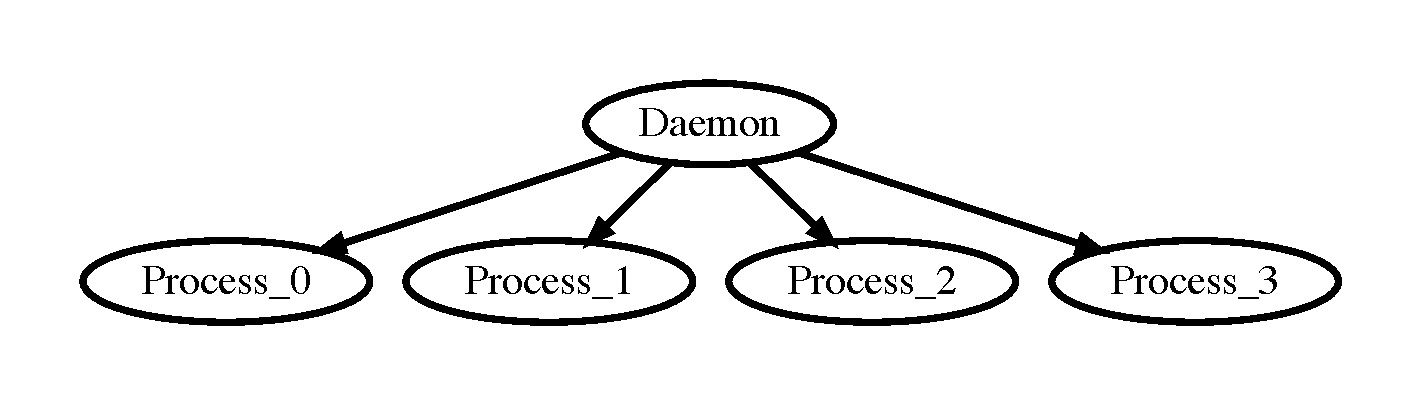
\includegraphics[width=\linewidth]{server_client.pdf}
  \caption{Hierarchical notification of hosted processes through \pmix notification routines. The \prrte daemon is in charge of observing, and forward notifications to the node-local managed application processes. The detection and reliable broadcast
  topology operates at the node level between daemons.}\label{fig:hosted}
\end{figure}

To detect process failures that are not congruent with a node failure, we
leverage on the direct observation of application processes that can be
performed by the node-local daemon. Since a process failure does not
impact the execution of the runtime daemon managing that process, that
daemon can execute localized observation strategies which are dependent
upon node-local operating system services. For example, the \orte Daemon
Local Launch Subsystem (ODLS) monitors SIGCHLD signals to detect discrepancies
in the core-binding affinity with respect to the user requested policy.
%Before the children processes execute the targets' executable, it need to set affinity of children processes according to a complex series of rules. This binding may fail in a myriad of different ways, the children processes will send a message to the parent indicating what happened (rendered error message) and the parent will read the message and analyze if this is a process failure and then use the runtime system's reporting mechanisms to display this error globally.
That same signal also permits, from the node-local daemon, an extremely fast and efficient observation
of the unexpected termination of a local application process. As a substitute,
or in complement, a daemon may also deploy a watchdog mechanism~\cite{CASTAIN18}
to capture non-terminating crash failures that may arise from software
defects, like live-locks, deadlocks and infinite loops.

\subsection{Detection of Node/Daemon Failures}

Resilient \prrte's algorithm for node/daemon failure detection has two
components: a node-level observation ring, and a reliable broadcast overlay network between daemons.

We arrange all N daemons to a logistic ring topology, as illustrated in Figure~\ref{fig:Ring}.
Thus, initially, each daemon \textbf{\textit{d}} observes its predecessor $d-1 \mod{N}$ and is observed by
its successor $d+1 \mod{N}$. The predecessor periodically sends heartbeat messages to \textbf{\textit{d}} (with a
configurable period $\delta$). At the same time, \textbf{\textit{d}} sends heartbeat messages to its own observer. For each node, a daemon emits heartbeats $m_1$, $m_2$, ... at time $\tau_1$, $\tau_2$, ... to its observer \textbf{\textit{o}}. Let $\tau_i' = \tau_i + t$. At any time \textbf{\textit{t}} $\in [\tau_i', \tau_{i+1}')$, \textbf{\textit{o}} knows that \textbf{\textit{d}} is alive if it has received the
heartbeat message $m_i$ or higher. Otherwise, \textbf{\textit{o}} suspects that \textbf{\textit{d}} has failed and initiates the propagation of the
failure of \textbf{\textit{d}}.

\begin{figure}[h]
\centering
\begin{minipage}[t]{.22\textwidth}
  \centering
  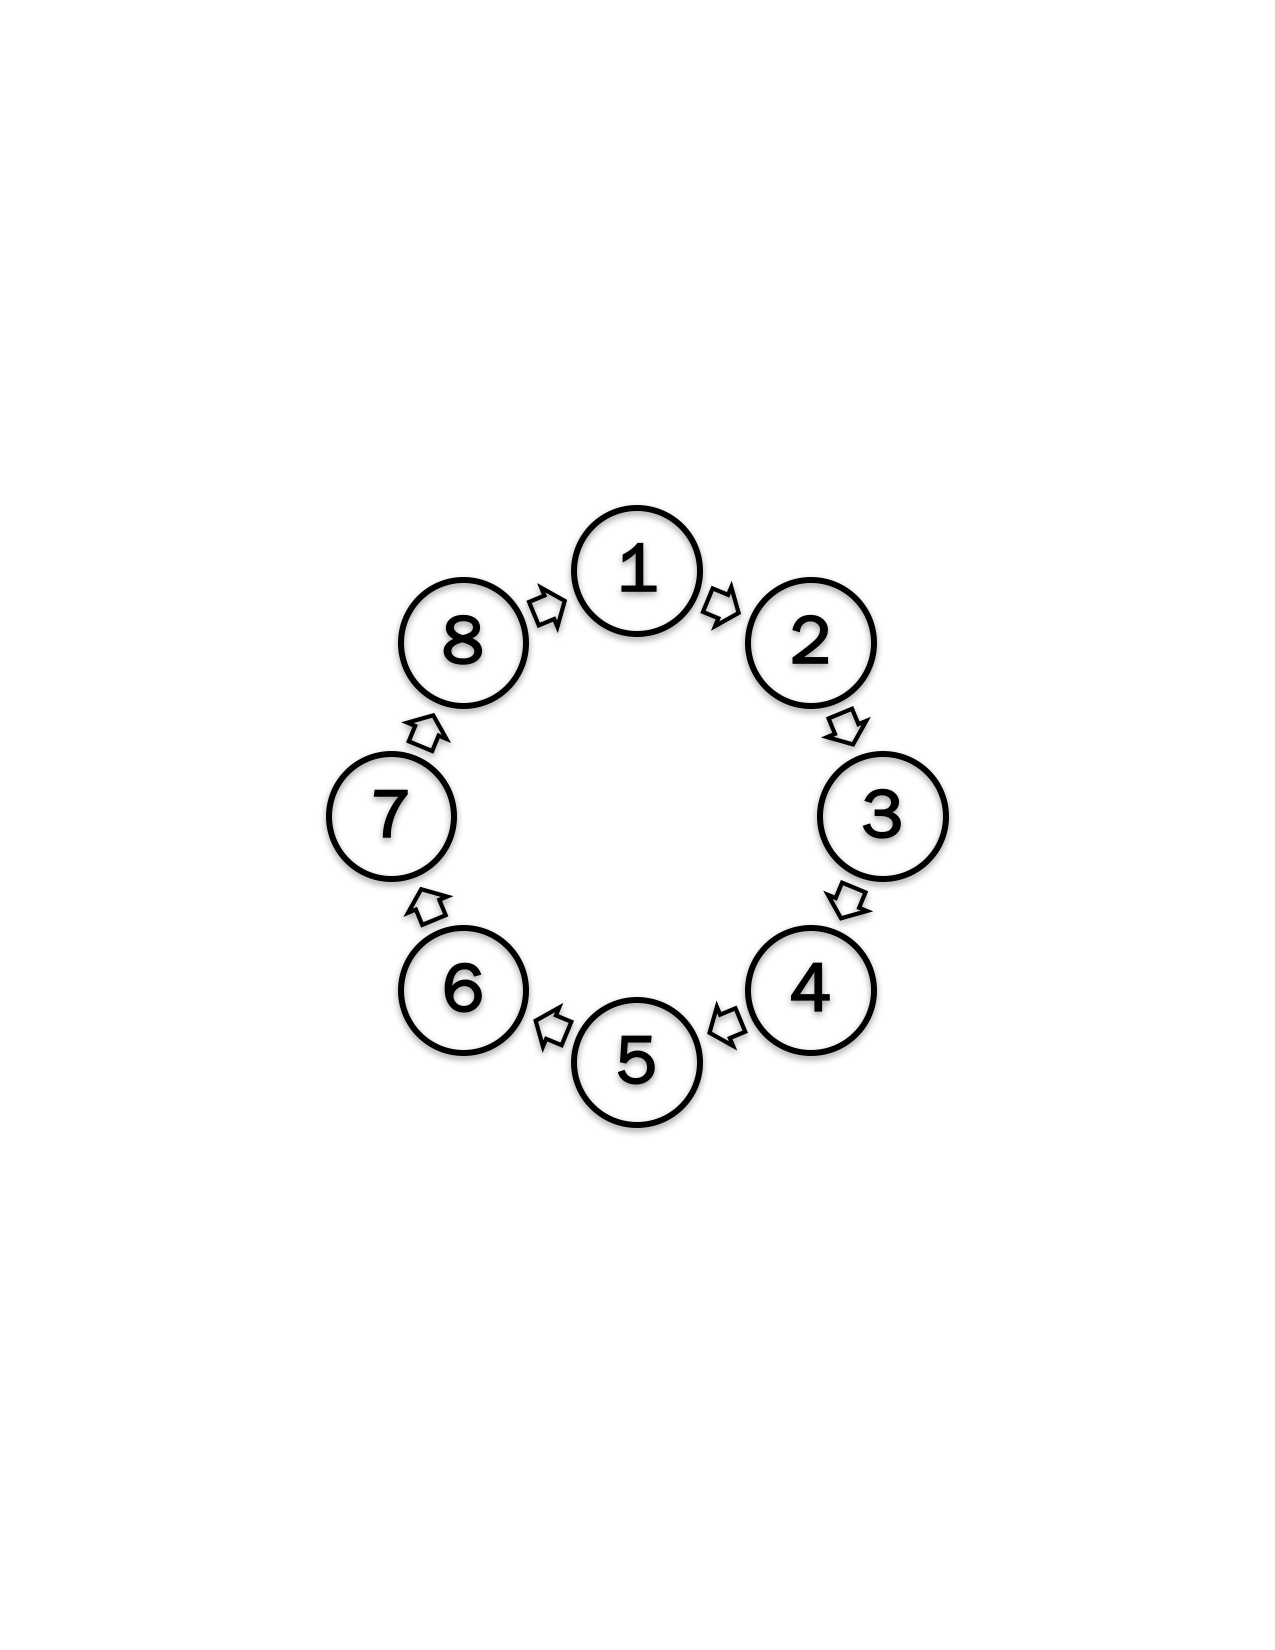
\includegraphics[trim=3cm 8.0cm 3cm 8cm,width=\linewidth]{ring_detector.pdf}
  \captionof{figure}{Daemons monitor one another along a ring topology to detect node failures.}
  \label{fig:Ring}
\end{minipage}%
\hfill
\begin{minipage}[t]{.22\textwidth}
  \centering
  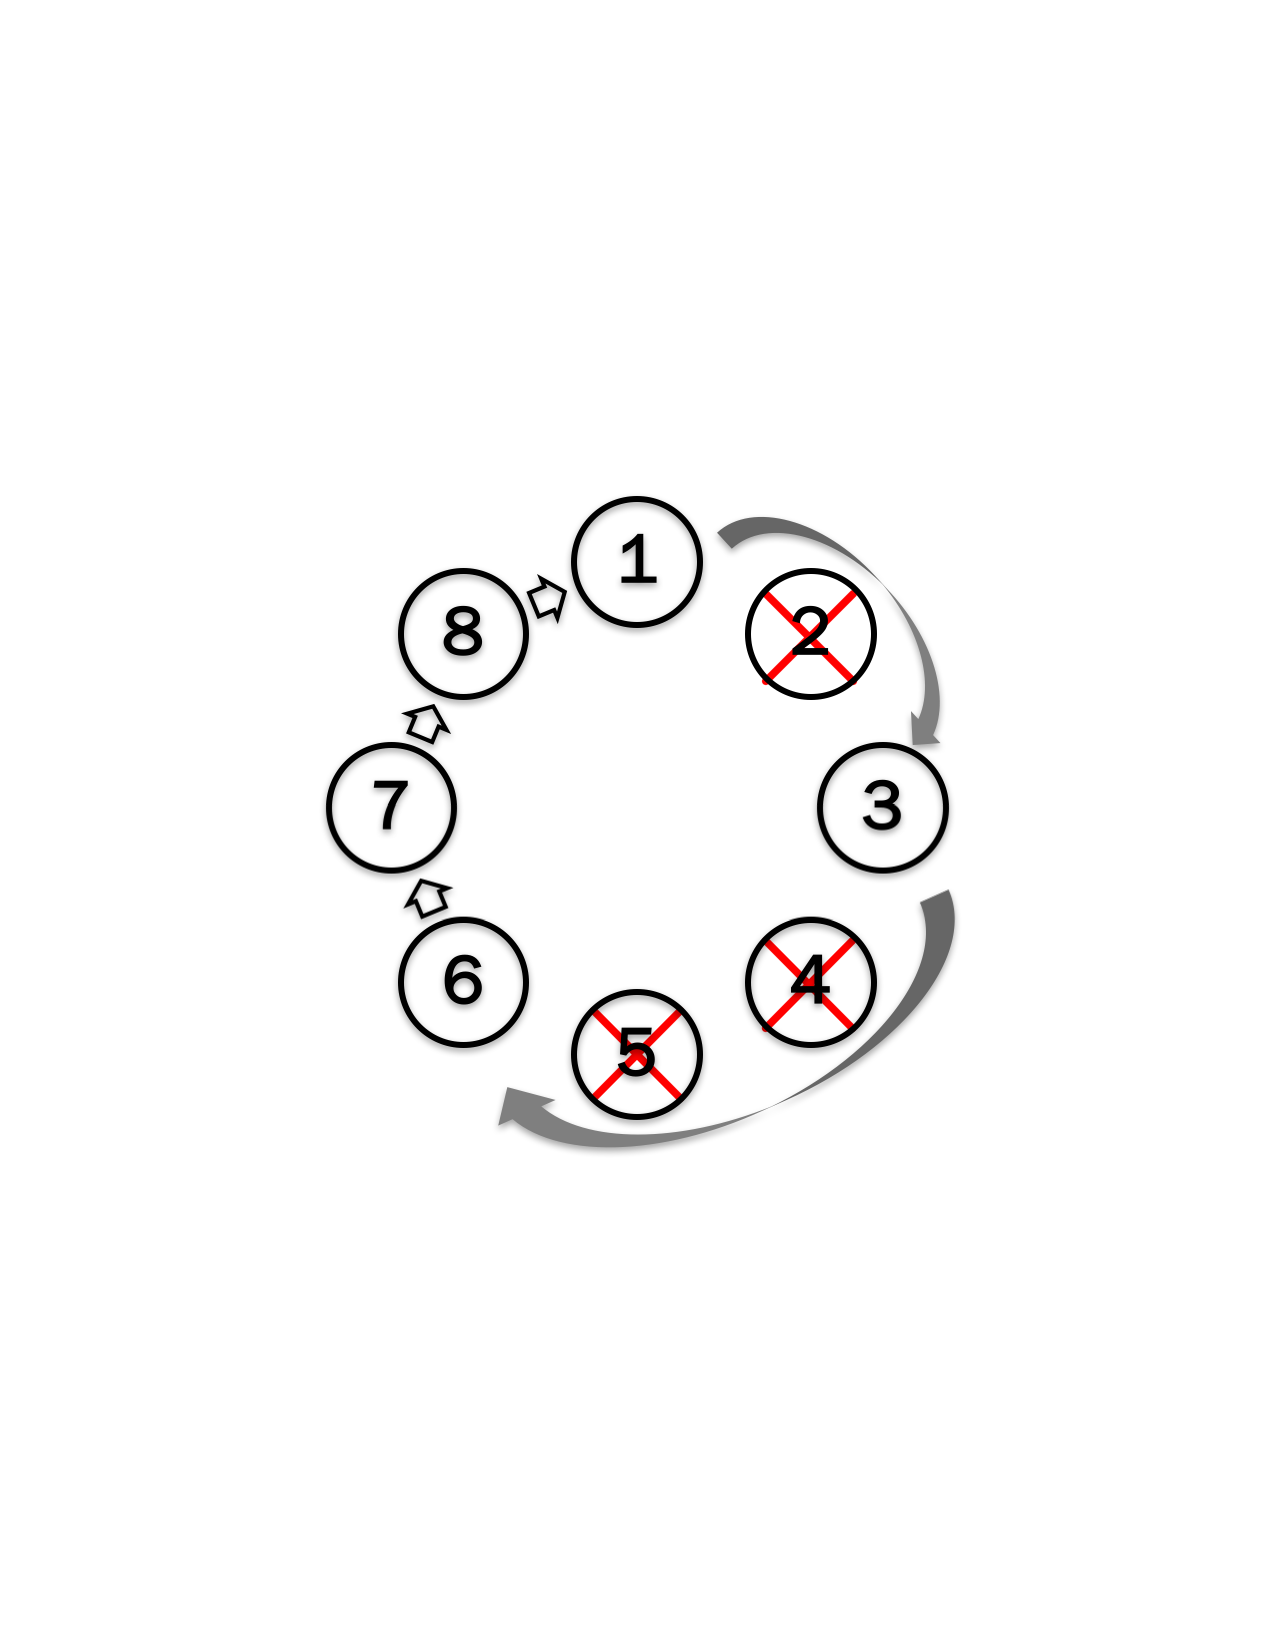
\includegraphics[trim=3cm 8.0cm 3cm 8cm,width=\linewidth]{reconnet_cross.pdf}
  \captionof{figure}{The algorithm mends the detection ring topology when a node failure occurs by requesting heartbeats from the closest live ancestor in the ring.}
  \label{fig:ReconnectRing}
\end{minipage}
\end{figure}

When the observer detects that its predecessor has failed, it undergoes two major steps.
First it needs to reconnect the ring topology, as illustrated in Figure~\ref{fig:ReconnectRing}. Daemon \textbf{\textit{o}} tries to
observe the precedessor of \textbf{\textit{d}} (the daemon it previously observed).
It sets \textbf{\textit{d-1}} as its new predecessor and then send a request to \textbf{\textit{d-1}} to initiate heartbeat emission. Of course,
it is possible that \textbf{\textit{d-1}} has also failed, which will be detected at the next timeout. In order
to speedup the reconnection process, \textbf{\textit{o}} may skip over
daemons that have already been reported as failed in the past (i.e., daemons
whose identifier is in $Reported_o$ because they have been observed and reported
by another daemon). Each time a daemon is marked as failed, all the processes it
managed are also marked as failed. After we get the list of all those affected processes and nodes, the observer component calls the propagation component to broadcast the fault information to other daemons, and then notify its local processes.

  %For all those nodes who received the notification, each node need to forward this information, maintain its own List\{\textit{ID}\} and notify locally. As show in figure \ref{fig:prrte}, we create a new module in error management as detector to enable this feature.

\subsection{Broadcasting Fault Information}
Considering that the observation topology is static, it does not provide
automatic or probabilistic dissemination of fault information. Thus, to complete
the reporting of failures, failures identified by an observer must be broadcasted
to inform all other daemons and application processes. An important aspect,
when considering a runtime that tolerate node/daemon failures, it that the
propagation algorithm itself needs to be resilient to failures.

For broadcasting fault information between daemons, we use the scalable and fault
tolerant BMG topology~\cite{Angskun07}. BMG has good fault-tolerant properties such
as optimal connectivity, low fault-diameter, strongly resilient and good optimal
probability in failure cases. Note that unlike prior works, the propagation
algorithm~\ref{fig:2lvlbmg} is not a flat BMG when application processes are considered, but consists of an
inner BMG overlay between daemons, and an outer star overlay from each daemon to its
local managed processes.

\begin{algorithm}
\caption{Two-Level Reliable Broadcast Algorithm}\label{fig:2lvlbmg}

\textbf{\textit{N}} \Comment{Number of nodes (value from environment)}\\
\textbf{\textit{Eid}} \Comment{Identifier of a process observed as failed (input parameter)}\\
\textbf{Reported$_i$} \Comment{Set of identifiers of previously reported failures, local to daemon \textbf{i} (initially empty)}\\
\textbf{\textit{msg}} \Comment{Message containing the set of process identifiers to report (initially empty)}\\
\textbf{Hosted\{$Did$\}} \Comment{Set of process identifiers managed by
the daemon $Did$ (initially empty, obtained from environment)}\\

\begin{algorithmic}[1]
\Procedure{StartPropagation}{ $Eid$ } \Comment{Daemon \textbf{j} starts the propagation}
\If {( $Eid$ $\notin$ $Reported_i$ )}
  \State Add $Eid$ to $msg$
  \If {$Eid$ is a daemon}
    \State Obtain $Hosted\{Eid\}$
    \State add $Hosted\{Eid\}$ to $msg$
  \EndIf
  \State ReliableBroadcast( $i, N, msg$ )
  \State Add $msg$ to $Reported_i$
\EndIf
\EndProcedure
\end{algorithmic}

\begin{algorithmic}[1]
\Procedure{ReliableBroadcast}{ $i, N, msg$ } \Comment{Daemon \textbf{i} sends error messages to all its neighbors}
\For{ $k \gets 0$ to $\log_2 N$ } \Comment {Neighbors in the BMG}
  \State {\textbf{i} sends \textbf{msg} to  ( ($N$ + i + $2^k$) \textbf{mod} {N} ) }
  \State {\textbf{i} sends \textbf{msg} to  ( ($N$ + i - $2^k$) \textbf{mod} {N} ) }
\EndFor
\ForAll{ $lp \in Hosted\{i\}$ } \Comment {Local application processes}
    \State {\textbf{i} sends \textbf{msg} to \textbf{lp}}
\EndFor
\EndProcedure
\end{algorithmic}

\begin{algorithmic}[1]
\Procedure{Forwarding}{ $msg$ } \Comment{Triggered when daemon or process \textbf{j} receives $msg$; decides if the message needs to be forwarded and notified locally}
\If {$msg \not\subset Reported_j$}
    \If {$j$ is a daemon}
        \State ReliableBroadcast( $j, N, msg$ )
    \EndIf
    \State Add $msg$ to $Reported_j$
\EndIf
\EndProcedure
\end{algorithmic}

\end{algorithm}

Figure~\ref{fig:bmg} shows an example of the execution of the BMG broadcast
with 12 nodes. For simplicity, the local start stemming from each daemon are not
represented.

\begin{enumerate}
 \item In this example, daemon 0 is the initial reporter and its observer component starts the propagation by calling the \textsc{StartPropagation} reliable broadcast algorithm.
 \item This prepares a broadcast message containing the identifier of the
 failed process (or daemon), and the associated application processes, when relevant.
 daemon 0 issues the message to its neighbors in the BMG topology.
 \item Upon receiving a broadcast message, a daemon considers if the message needs
 to be forwarded. If the message carries a list of processes that are already known to
 have failed, then, the daemon already triggered the propagation, and no further
 action is needed. Thus every daemon forwards the message once, insuring that
 all edges of the BMG will carry exactly one message per detection.
\end{enumerate}


\begin{figure*}[ht!]
  \begin{minipage}{.45\textwidth}
    \centering
    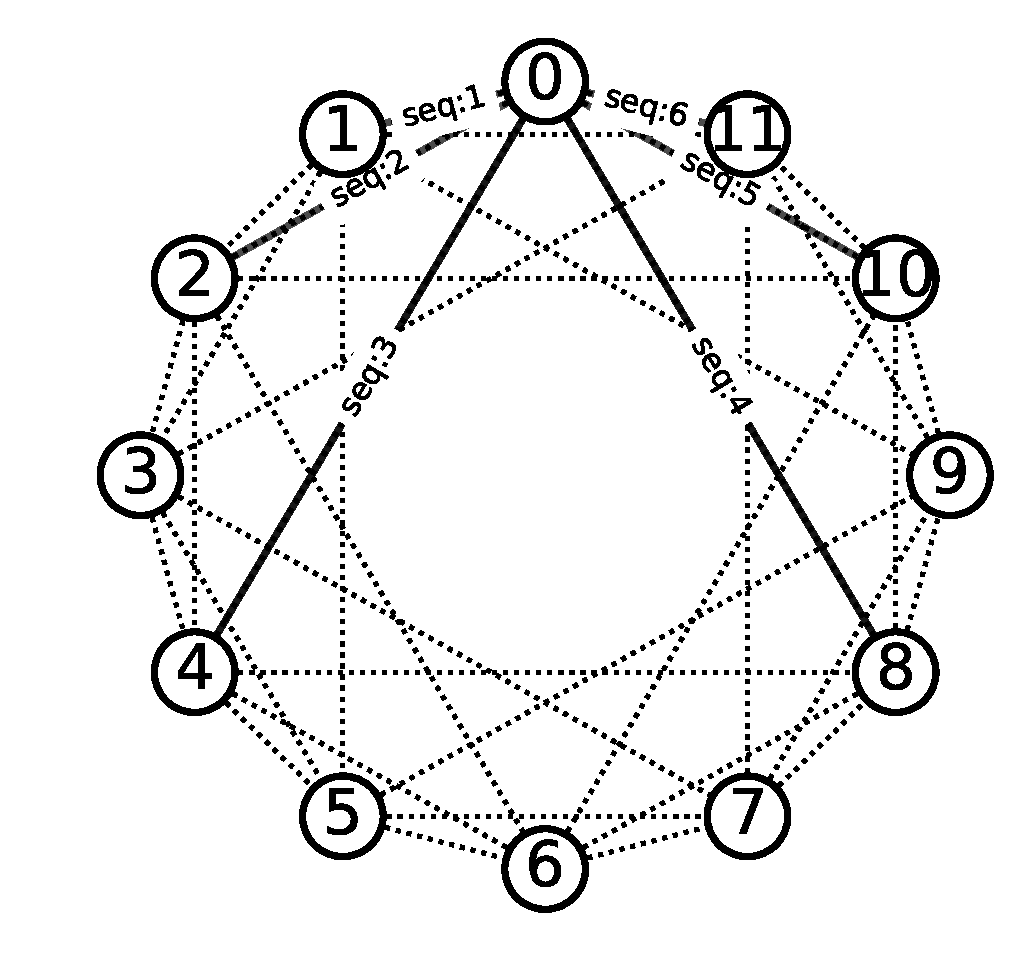
\includegraphics[scale=.3]{BMG_seq.pdf}
    \caption{Binomial graph with 12 nodes}
    \label{fig:bmg}
  \end{minipage}
  \begin{minipage}{.45\textwidth}
    \centering
    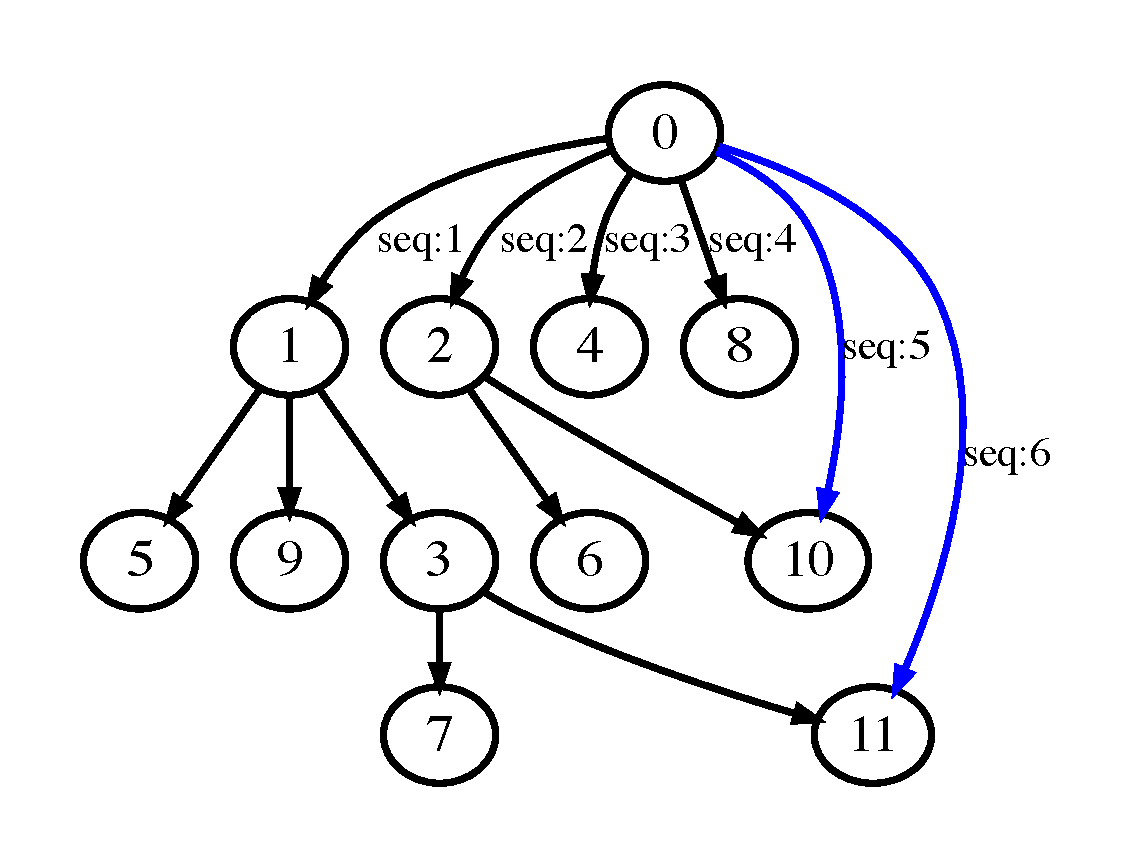
\includegraphics[scale=.3]{reorder_span.pdf}
    \caption{Broadcast using binomial spanning tree from node 0, extra messages to neighbours are colored in blue}
    \label{fig:reorder_span}
  \end{minipage}
\end{figure*}

The propagation message issued at each daemon are ordered so that the
messages that are part of a binomial spanning tree rooted at the emitter
are sent first. Figure \ref{fig:reorder_span} shows the a spanning tree
for a broadcast originating from node 0; the extra messages (5 and 6, colored
in blue) are supplementary messages that provide redundancy and ensure that
any node in the BMG can always be reached within $O(log_2 N)$ steps (given
that less than $2 log_2 N$ failures strike, with more failures,
statistically rare scenarios can degenerate in a linear propagation time).
The advantages of this new broadcast algorithm are:
\begin{enumerate}
  \item Sequence ordering brings higher parallelism: messages to node \{10, 11, 7\} could arrive from any redundant forwarding path rather than only from the 0-rooted spanning tree. This may decrease the apparent height of the tree, the average latency and thus reduce the average notification latency.
  \item Limited network degree: the maximum degree for every daemon is logarithmic, which avoids hot-spot effects that are common in randomized gossip algorithms.
  \item Deterministic number of messages: the total number of messages is
  exactly the number of links in the BMG topology, that is, $O(N log_2 N)$
  messages overall. In contrast, random march gossip algorithms have to
  balance the overall
  \item Number of heartbeats and propagation messages is dependent Upon
  the number of nodes, not the number of managed application processes.
  In manycore systems, this has the potential to significantly reduce the
  effective cost of the algorithm when compared to a flat topology between
  application processes.
\end{enumerate}

\begin{figure}[h]
  \centering
  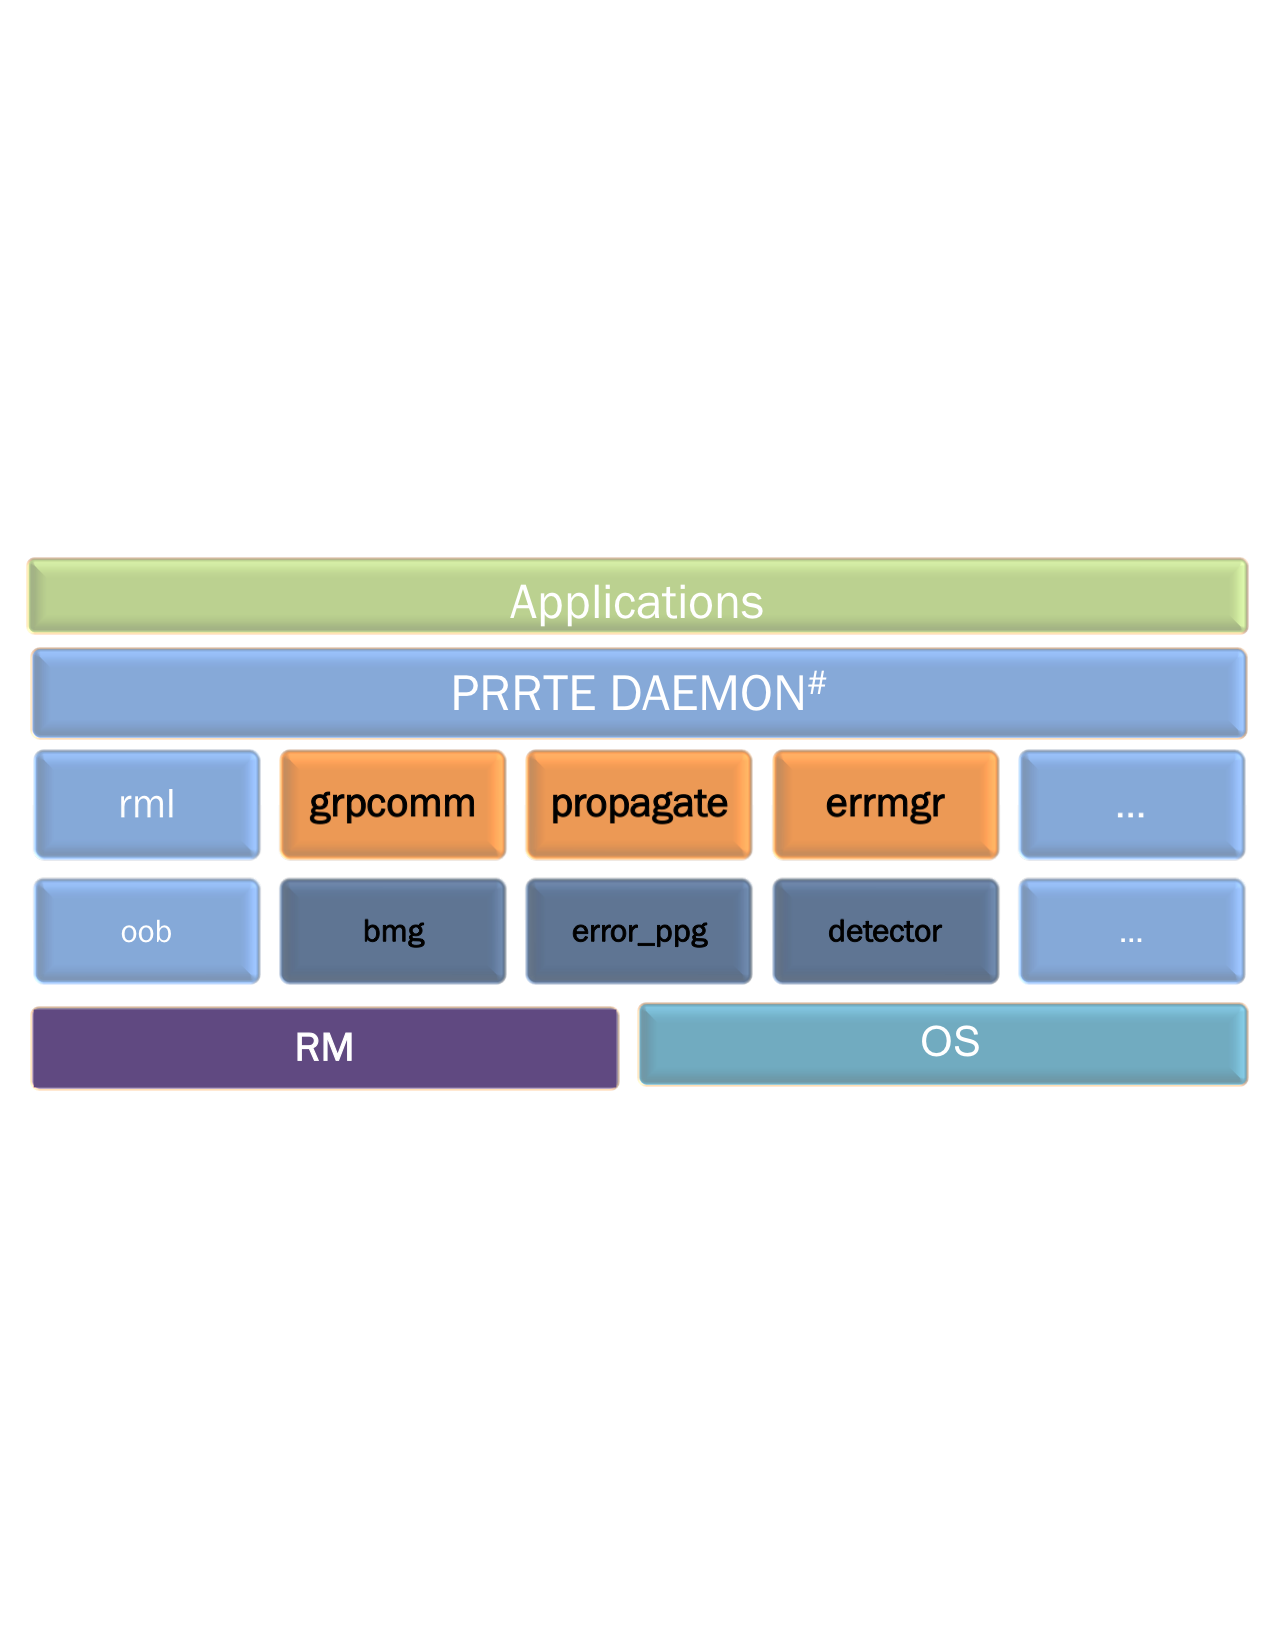
\includegraphics[trim=0.2cm 9.0cm 0.2cm 9cm,width=\linewidth]{PMIx_PRRTE.pdf}
  \caption{Resilient \prrte component architecture. The orange boxes represent the component we mainly use to add the resilient features. The dark blue colored boxes are new modules}\label{fig:prrte}
\end{figure}

\subsection{Implementation}

\todo{this paragraph too verbose}

\subsubsection{\pmix Interface}
We implemented \ourwork as a set of components in \prrte. \prrte is a fork of the \ompi runtime, \orte~\cite{Castain05}. \prrte is developed and maintained
by the \pmix community as a demonstrator and enabler technology that demonstrates
and exercises the features of the \pmix interface~\cite{CASTAIN18} --an abstract set of interfaces by which not only applications and tools can interact with the resident system management stack (SMS), but also the various SMS components can interact with each other.
Many communication libraries, resource managers, and job scheduling systems are currently employing \pmix in production, and many more are under development.
For example, \ompi has now substituted \orte with a shim layer over \pmix and thus can be launched and monitored by \prrte.
Similarly, \oshmem uses \prrte as the default launcher.
Meanwhile, the Slurm batch scheduler and job starter ships with native \pmix support, meaning that an application that interoperate with Slurm through \pmix can be ported  over \prrte without effort.
Overall, the fact that \prrte interfaces with the communities of interest
highlighted in Section~\ref{sec:motivation} through a well defined and stable interface is a clear benefit for increasing the impact of \ourwork.

The \pmix specification provides a specified Job controlling and Monitoring interface~\cite{Ralph15} which (in theory) enables the application and SMS to coordinate the response to failure.
Another important feature is the \pmix Event Notification~\cite{Ralph002} : the resource manager or server can notify the application of events, the application processes can notify their server or SMS of issues.
The outputs of \ourwork are exposed to client libraries (e.g., MPI) through
these interfaces, and, to the best of our knowledge, \ourwork is the first
implementation to populate these interfaces with a truly resilient implementation.

Notifications of failures are produced as \pmix Event Notifications, which can be easily subscribed by the client or the SMS to track failures detected by \ourwork.
We also employ \pmix Even Notifications to perform the internal propagation of failure notifications between daemon processes and application processes.

\subsubsection{\ourwork in the \prrte Architecture}

While a full depiction of the architecture and feature set of \prrte is out of the scope of this paper, some are relevant to our implementation effort.
\prrte is based on a Modular Component Architecture (MCA) which permits easily extending or substituting the core subsystem with experimental features.
As shown in in figure~\ref{fig:prrte}, within this architecture, each of the major subsystems is defined as an MCA framework, with a well-defined interface, and multiple components implementing that framework can coexist.

We added two new frameworks and four components to \prrte daemons. The \texttt{proc\_failure}
component is in charge of detecting the failure of locally hosted processes (using
SIGCHLD signals from the operating system). The \texttt{BMG} components
implements a broadcast algorithm in a reliable way; to be noted, this component
abides by the normal interface for a daemon broadcast, meaning that it is not
limited to reliably broadcast fault information. The \texttt{detector}
component emits heartbeats and monitors timeouts, and last, the \texttt{error\_ppg}
components prepares the content of the reliable broadcast messages (i.e., the list
of failed processes).

An important aspect of the propagate framework is that, for node failures,
only the daemon that initiates the propagation needs to obtain the list of processes
hosted  by the failed daemon (line 5 of procedure \textsc{StartPropagation} in Algorithm~\ref{fig:2lvlbmg}).
Since only one process initiates a propagation, this information is obtained
 only once (using \pmix key-value store operations) and does not need to
 be replicated during initiation (memory overhead) or fetch on-demand from
 a large number of daemons (network hot-spot).

\begin{figure*}[h]
\centering
\begin{minipage}{.37\textwidth}
  \centering
  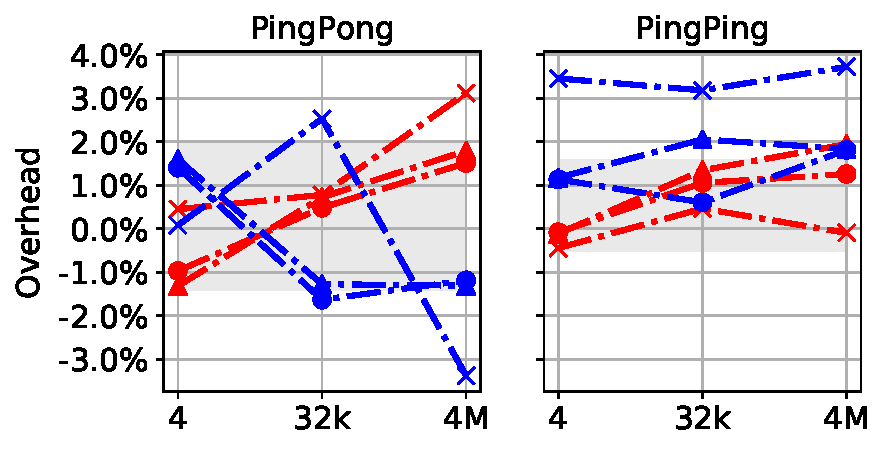
\includegraphics[width=\linewidth]{multi_pingping_pingpong_overhead.pdf}
\end{minipage}%
\begin{minipage}{.63\textwidth}
  \centering
  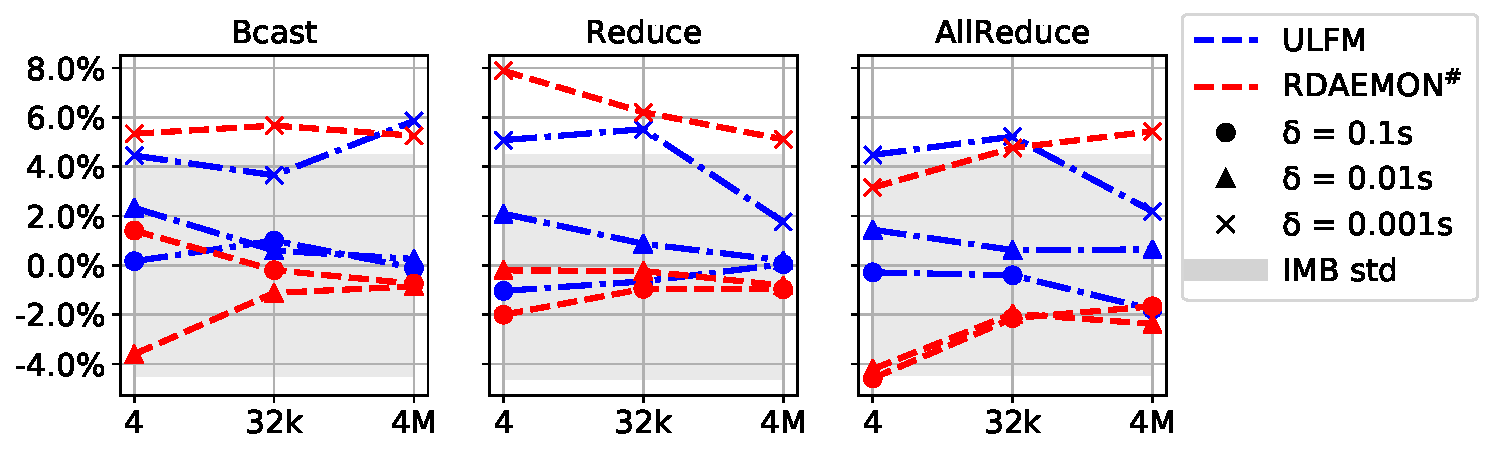
\includegraphics[width=\linewidth]{Bcast_overhead_with_ulfm_max_col.pdf}
\end{minipage}
\captionof{figure}{\prrte with fault tolerance overhead over \prrte and \ulfm using IMB}
\label{fig:overhead}
\end{figure*}

\section{Experimental Evaluation}\label{sec:experiments}

\subsection{Experimental Setup}
Experiments are conducted on two different machines: (1) ICL's NaCl is an Infiniband QDR Linux cluster comprising 66 Intel Xeon X5660 compute nodes, 12 cores per node; (2) NERSC's Cori
%~\cite{Cori01}
is a Cray XC40 supercomputer with Intel Xeon "Haswell" processors and the Cray "Aries" high speed inter-node network, 32 cores per node. Our \ourwork is based upon \prrte (\#71ef547), with external \pmix (\#21d7c9). We compare with \ulfm revision \#77f9157, which is based on the same base version of \ompi we use to evaluate \ourwork in MPI workloads. Each experiment is repeated 30 times and we present the average. We use Intel MPI Benchmark (\imb v2019.2)~\cite{IMB} for MPI performance measurements for point-to-point (P2P) and collective communications (one \mpi rank per core). For all experiments we use map-by node, bind-to core binding policy which puts sequential MPI ranks on adjacent cores. The only exception is the \imb P2P experiment where we use
the map-by node, bind-by node policy to set communicating \mpi ranks on different nodes.

\subsection{Accuracy}
\begin{figure}[h]
  \centering
  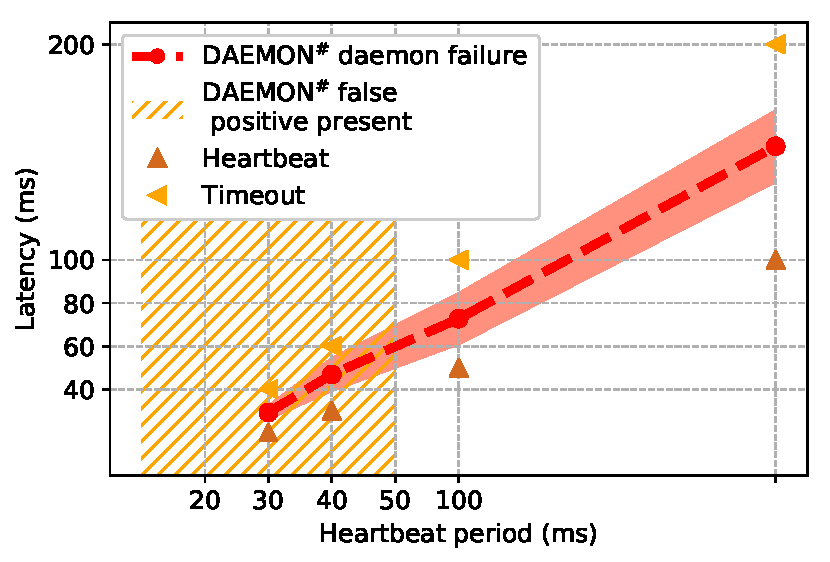
\includegraphics[width=\linewidth]{accuracy.pdf}
  \caption{Heartbeat and Timeout accuracy}
  \label{fig:accuracy}
\end{figure}

For the first experiment we want to explore the accuracy of \ourwork's detector with different heartbeat periods.
%
The accuracy experiment is conducted by (1) Starting with a large value for the
detection timeout $\eta$; (2) Verify that no failure is detected when there is no injection, and all injected failures are reported; (3) If the previous test is accurate, decrease $\eta$ (and accordingly the heartbeat period $\delta$) until we notice false positive detection. We set a constant ratio $\eta = \delta * 2$.
 %
 Figure~\ref{fig:accuracy} presents the results on NaCl 64 nodes.
 % For  non-communicating benchmarks (SETNAME\todo{name}), all tests succeed until $\delta$ is lower than 20 milliseconds.
 In heavily communicating Benchmarks
 (\imb point-to-point and collective tests), all tests succeed until the
  heartbeat period lower than 20 milliseconds. To further investigate,
  we measured that the heartbeat message is neither delayed by communication
  congestion nor compute pressure but we found out that daemons need some time to launch the processes when starting the job which causes false detection during job startup. \todo{remove the heartbeat accuracy, change timeout accuracy to 'false positive present'; for later: do not report finalize errors}

  %\item No failure is injected and node missed its heartbeat sending deadline. With a reasonable timeout value, all daemons can send heartbeats successfully with $ \delta $ as low as 0.1 millisecond.
%From all above we can see that the granularity of timeout is 40 milliseconds limited by the latency for daemons to launch the application processes. And the granularity of heartbeat period is 0.1 millisecond.

\subsection{Noise}
We also investigate the noise overhead incurred on an MPI application by the heartbeat emissions
and management from \ourwork.
Figure \ref{fig:overhead} illustrates the overhead incurred with P2P and collective communications running \imb.
%All IMB-MPI1 suits can be successfully conducted with no false detection with $ \delta \geq 1 ms $.
In order to contextualized the incurred overhead, we present in shaded grey the band of natural variability
of the benchmark without a failure detector active.
For the PingPong benchmark, we use the \texttt{-multi} mode of IMB with one rank per core on 2 nodes.
This ensures that all cores are active with the communication pattern and thus
compete for resources with \ourwork activities.
For the collective benchmarks, we run on 64 nodes using all cores. For each message size, we set the number of
repetitions for the test to last at a minimum 20 seconds so that multiple heartbeat emissions occur during the experiment. Overhead is calculated by using the maximum latency result, normalized by the non-fault tolerant performance:
\begin{equation}
Overhead = \frac{( {\ourwork - \prrte} )}{\prrte}
\end{equation}
 From the graph we can see that the latency performance and bandwidth performance are barely affected by heartbeats periods from milliseconds to seconds. Notably, when $ \delta \geq 10 ms $, it has trivial influence on the system, as illustrated by the fact that the average overhead is within the band of natural variability of the benchmark. When  $ \delta = 1 ms $ the noise in PingPong incurs less than three percent overhead. In collective communication the noise overhead is less than eight percent, slightly higher than the standard deviation of the benchmark itself at four percent.
 In a general comparison with \ulfm (normalized to its performance without failure detection active),
 We can see that \ourwork achieves a similar level of incurred noise for a given
 heartbeat period.

\subsection{Comparison with SWIM}
This section compares the failure detection latency and scalability of \ourwork with SWIM~\cite{Abhinandan02} --a random-probing based failure detection protocol and gossip membership updates. To decrease
the chance of false detection, SWIM uses a suspicion mechanism. When a node does not reply to a probing in time, the initiator then judges this node as suspicious (but not yet failed). It then broadcasts
\begin{figure}[h]
  \centering
  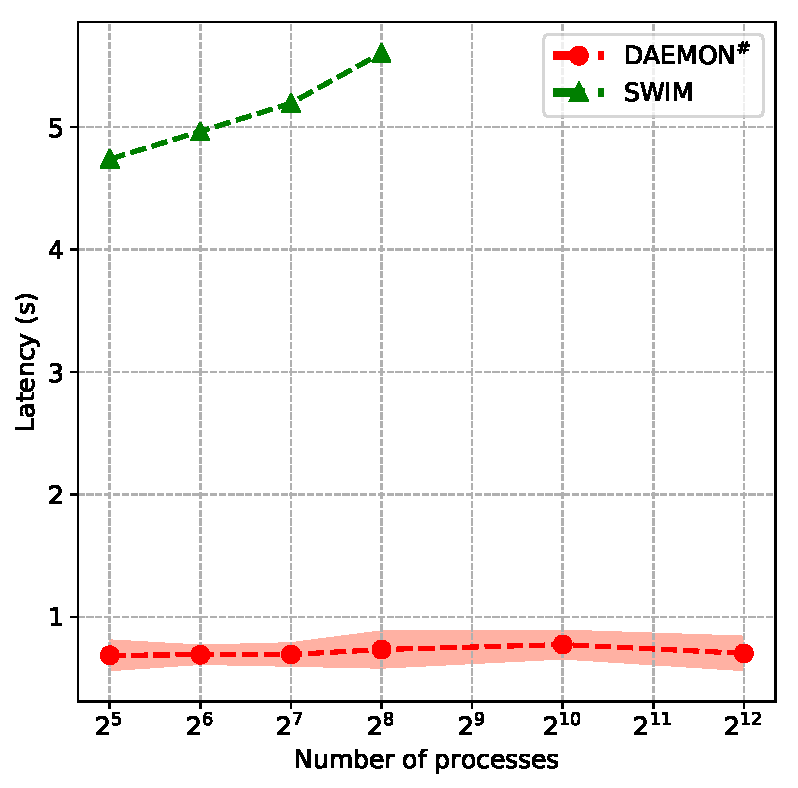
\includegraphics[width=\linewidth]{Scale_prrte_swim.pdf}
  \caption{Detection latency comparison between \ourwork and SWIM with increasing number of processes ($\eta=0.5s)$}
  \label{fig:scale_swim}
\end{figure}
this suspicion information within a subgroup, if any node in the subgroup receives an acknowledge before the timeout, it will declare the suspected node as alive, otherwise declare a failure. In order to improve the efficiency of multi-cast, SWIM uses an infection-style dissemination mechanism where information spreads in a manner analogous to the spread of gossip in society, or epidemic in the general population.
For the SWIM implementation, we use Go-Memberlist (\#a8f83c6). We used a go-\mpi interface
to replicate our \mpi detection benchmark with SWIM.

\begin{figure}[h]
  \centering
  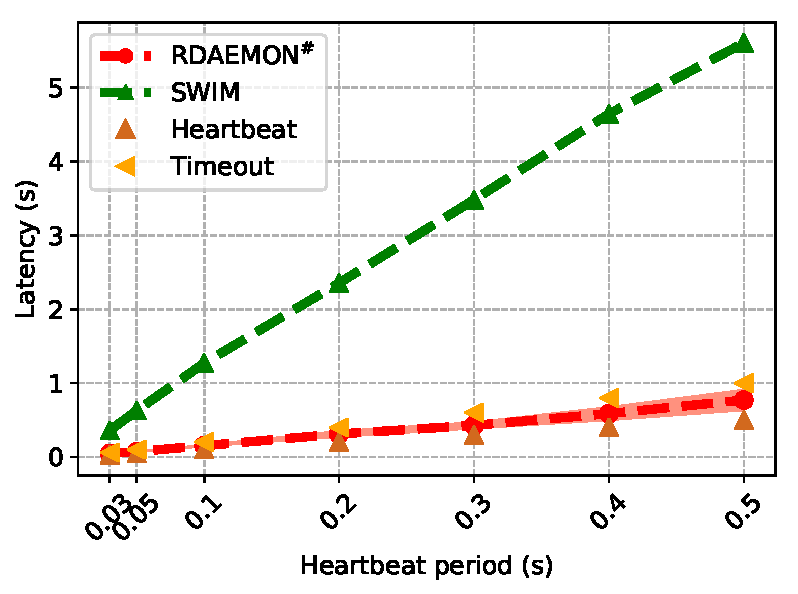
\includegraphics[width=\linewidth]{HB_prrte_swim.pdf}
  \caption{Detection and Propagation delay comparison betwern \ourwork and SWIM with varying heartbeat periods}
  \label{fig:hb_prrte_swim}
\end{figure}


Figure \ref{fig:scale_swim} compares the scalability of the two detectors with regard to the number of deployed processes with $\eta = 0.5s$, $\delta = 1s$.
%For smaller number of processes is stabilizing in approximately 0.75s, while the stabilization delay of SWIM is 5s.
We could run SWIM tests only up to 256 members, after that limit, some nodes exceed the maximum connection backlog
set in the operating system for \texttt{listen} operations on TCP sockets, causing an application crash during
initialization. For \ourwork,
% we also synchronize with barrier, and then inject node failure, detection and notification latency is collected on each process.
we run all tests up to 768 processes on 64 nodes.
%
As the number of processes increases latency of \ourwork remains almost the same.
For 4K processes, the stabilization of \ourwork is still below the range of the heartbeat period and timeout.
SWIM latency shows a linear increase when the number of processes increase which will be the bottleneck when scaling up (assuming the maximum connection requests limit issue can be solved).

Figure~\ref{fig:hb_prrte_swim} compares single node failure detection and propagation latency between \ourwork and SWIM\todo{how many nodes/processes in that experiment?}
with different heartbeat periods setting. For all tests we set $ \eta = \delta * 2 $. We can clearly see that for \ourwork the detection latency is between ($\delta$, $2*\delta$), and the last notification happens very soon after the detection, which demonstrate the efficiency of our propagation algorithm (variability in the results comes from the randomness of when the node failure happened with respect to the heartbeat period). However, for SWIM, even with smaller number of processes the latency is still more than $10*\delta$, because after the initial timeout declares a suspicion, the gossip protocol and confirmation mechanism have to be executed
before the failure is reported.

\subsection{Comparison with \ulfm for Process Failures}
This section compares \ourwork with the other extreme on the spectrum of
general versus specialized; \ulfm. The \ulfm implementation also has two
 main components: process level detection ring, and propagation overlay with all launched processes. The detection ring is built at Byte Transfer Layer (BTL) level - which provides the portable low-level transport abstraction in \ompi. \ulfm's current implementation provides several mechanisms to ensure the timely activation and delivery of heartbeats:
\begin{enumerate}
  \item Using a separate, library internal thread to send the heartbeats in order to be separated from the application's communication. This also mitigates the drift in heartbeat
  emission dates (which would cause false positive detection) in compute intensive application.
  For receiver it need to poll BTL engine to check the aliveness of its successor.
  \item Using RDMA put to raise a flag in the receiver's registered memory. by using the hardware accelerated put operations, \ulfm avoids the problem of active polling BTL engine.
  \item Using in-band detection directly from the high performance network
  fabric to report unreachable error directly to the propagation component.
\end{enumerate}

\begin{figure}[h]
  \centering
  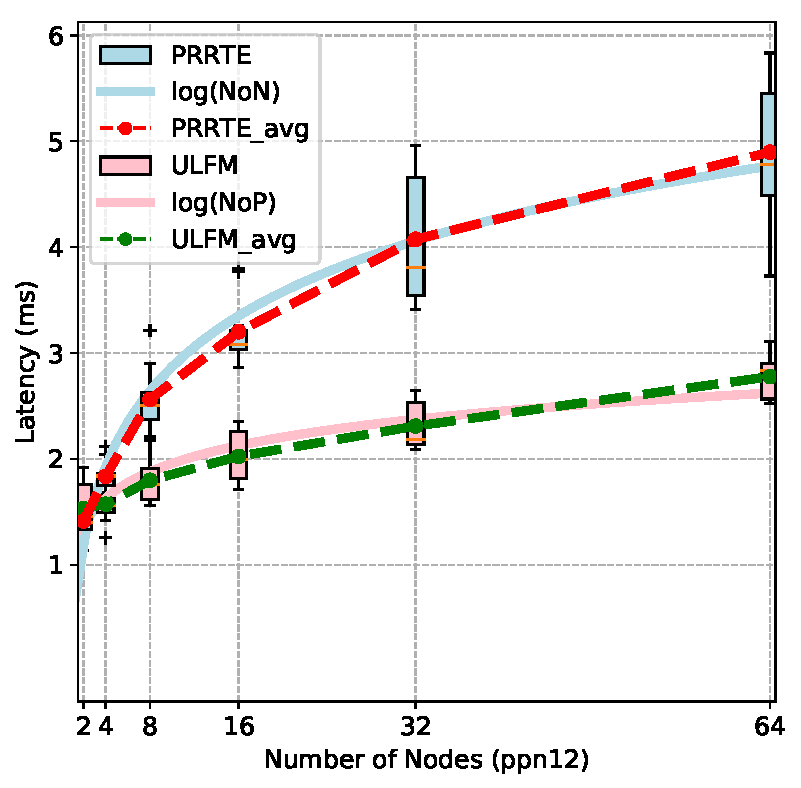
\includegraphics[width=\linewidth]{Process_Failure_log_fit.pdf}
  \caption{Process failure detection and propagation delay compared to \ulfm}
  \label{fig:proc_failure_nacl}
\end{figure}

The propagation overlay is also built at the BTL level. Reliable broadcast
messages are sent using the same active message infrastructure employed to
deliver short \mpi messages and matching fragments (however, a different
tag is employed to avoid disrupting the \mpi matching). Because the
propagation happens at the application process level, all \mpi processes
are part of the reliable broadcast algorithm, thus the lower bound for reaching
all processes is $\log_2({Number\ of\ Processes})$.

In contrast, \ourwork process failure detection is implemented at the daemon
level. This mechanism doesn't pressure the application communication resources,
and can progress the processing of heartbeats without the need for
RDMA hardware. The broadcast overlay in \ourwork is built at the daemon
level which decreases the number of participants to the number of nodes, a potentially
large saving in manycore systems. This helps reduce
the total messages transferred and forwarded compared to \ulfm, and the
 the lower bound for a full propagation is $\log_2({Number\ of\ Nodes})$.

\begin{figure}[h]
  \centering
  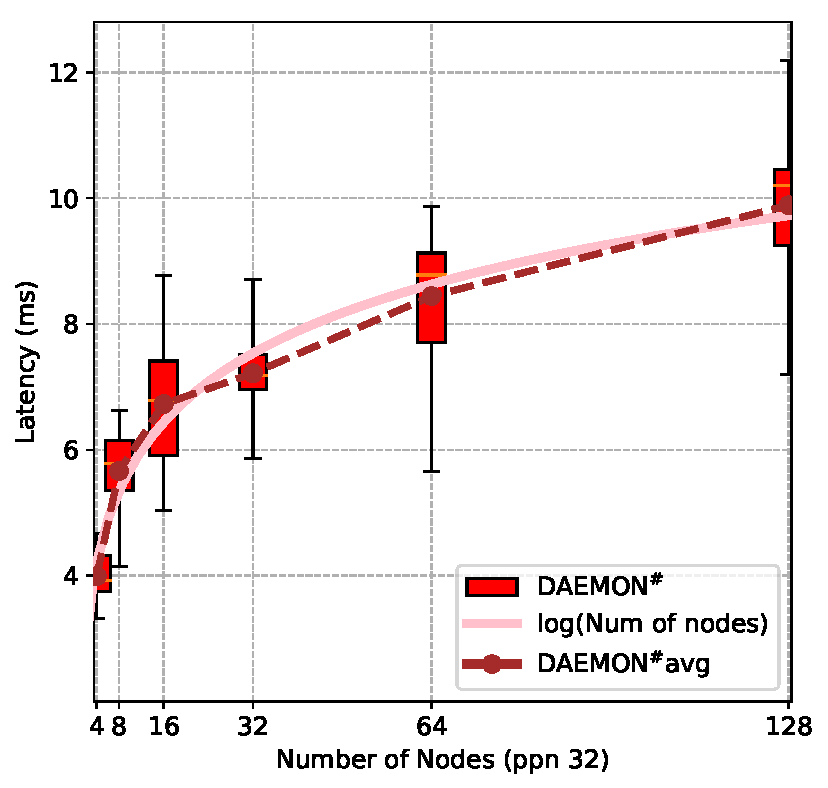
\includegraphics[width=\linewidth]{Cori_Process_Failure_fit.pdf}
  \caption{Process failure detection and propagation delay on Cori}
  \label{fig:proc_failure_cori}
\end{figure}

Figure~\ref{fig:proc_failure_nacl} compares the latency of process failure detection and propagation of \ulfm and \ourwork. The sensitivity of \ulfm heartbeat without false detection is 10 milliseconds, but we want to compare the best performance from \ulfm using high speed in-band detection which is faster than using the lowest heartbeat period. For \ourwork, the daemons are in charge of detecting process failure. \ourwork uses TCP to broadcast among daemons, daemons use \pmix's notification method to distribute the error information to all hosted processes. Experiments are conducted on NaCl from 2 nodes to 64 nodes using all cores on each node.
The process mapping results in \ulfm  using the in-band shared communication for detection and propagation\todo{did not understand that}. We can see that our implementation enjoys the same performance as \ulfm but highly reduced the complexity. The detection and propagation time is less than 5 milliseconds despite using TCP. For \ulfm the detection and propagation delay increases from 2 milliseconds to 3 milliseconds as the  number of processes increase. For both \ourwork and \ulfm the latency increase trend fit $ a*\log_2(N) + b $, which can be easily scale up to hundreds of thousands of nodes, but for \ulfm
the trend follows the number of processes rather than the nunber of nodes. Figure~\ref{fig:proc_failure_cori} scales the evaluation of \ourwork on the larger Cori system (with more processes per node). We can see that with 4K processes the detection and propagation latency is about 10 milliseconds, and the scalability trend remains logarithmic with the number of nodes (not processes).

\subsection{Node Failures Detection}
We now compare the detection latency for full-node failures. In \ourwork
node failures result in the loss of a daemon, for \ulfm they result in
the loss of multiple consecutive processes in the ring topology. In
both cases, the node failure is detected by the absence of heartbeats
before the timeout expiration.

\begin{figure}[h]
  \centering
  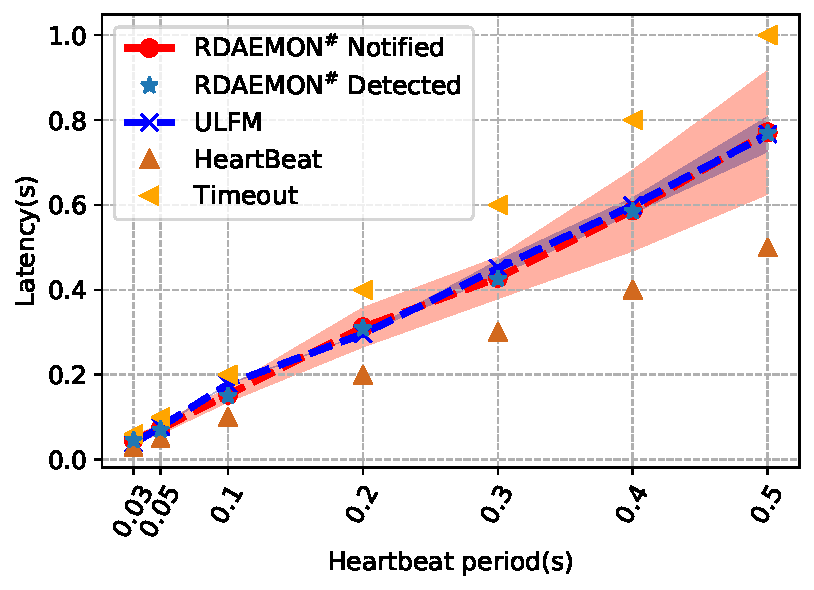
\includegraphics[width=\linewidth]{PRRTE_ULFM_comparision.pdf}
  \caption{Single Daemon Failure detection and propagation delay compared to \ulfm with different heartbeat period}
  \label{fig:node_failure_hb}
\end{figure}

Figure~\ref{fig:node_failure_hb} presents the behavior observed when injecting single daemon failure under different heartbeat period setting. We conducted the experiments on 64 nodes with 764 processes. For \ourwork after synchronizing, we inject a node crash by ordering a process to kill its host daemon. For \ulfm,
all application processes on the target node suicide as a group.
%However, \ulfm doesn't have the capability of detecting node failure, we simulate "node crash" by kill the last process on that node. With the process ring detector this particular process failure will be detected by its observer on another node, this behavior is the same as \ourwork's node to detect node failure.
%Also we assume that the time different between the daemon failure and process failure is trivial which is confirmed later in the experiment.
For the heartbeat period setting we start at 30 milliseconds to 0.5 second for both \ourwork and \ulfm. For all heartbeat periods we set $ \eta = \delta * 2 $. From the figure we can see that the detection latency in all cases lands in the interval $[\delta,\eta]$.

Figure \ref{fig:daemon_failure_diffnode} shows single node failure detection and propagation performance with a fixed heartbeat period $ \delta = 0.5s $ and an increasing total number of nodes. After a node crash, all processes hosted on this node will be affected, the observer node fetches and packs the information of all affected processes information then distribute the packed message.
\textbf{
\begin{figure}[h]
  \centering
  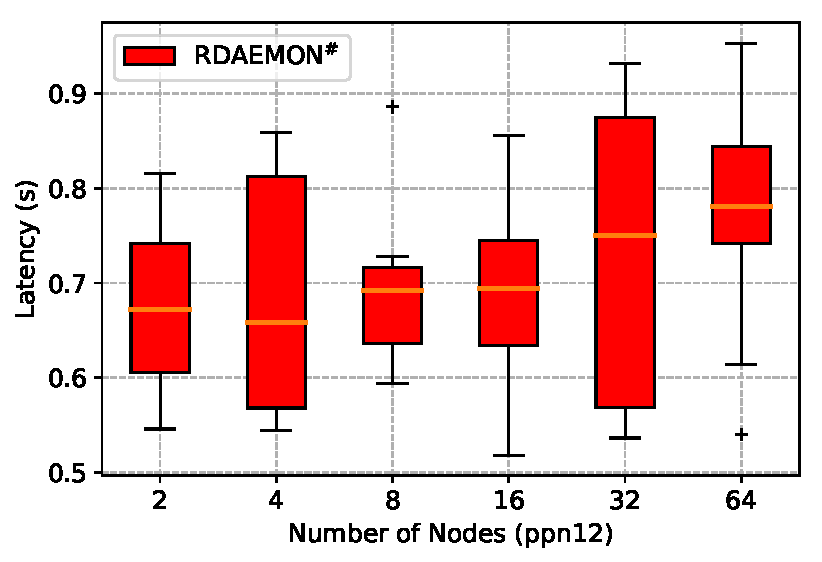
\includegraphics[width=\linewidth]{Daemon_prrte_only.pdf}
  \caption{Single Daemon Failure Detection and Propagation delay with different number of nodes}
  \label{fig:daemon_failure_diffnode}
\end{figure}}
%
\todo{the following paragraph seem to not describe what's on the graph anymore}
However, for \ulfm all affected processes need be detected by their observers independently, this will suffer from the collisions on the reliable broadcast propagation. For the worst case detection, all affected processes are adjacent in the observation ring, for each affected process the ring need to re-connect and update, causes a linear increase of $ \eta $ to the detection latency for every process failure. From the figure see that \ourwork can detect and propagate a node failure between (0.5s, 1s) for all tested number of node.
%

The last experiment, presented in Figure~\ref{fig:multi_daemon_failure_nacl}), investigates the effect of multiple concurrent node failures. The experiment is similar to the single node failure case, except for the
number of processes that inject failures. In the first scenario, we inject failures at random nodes.
In this case, the detection and propagation are independently conducted by different observer nodes and neatly overlap resulting in a marginal increase in the overall detection latency for
reporting all failures. We also consider the worst case scenario, in which failures strike
contiguous nodes. In this case, the daemon that detects the first failure
undergoes the ring-mending operation, which entails a linear number of timeouts
before all failures are reported. This indicates that, from a fault
tolerance perspective, the ordering of
daemons on the detection ring should avoid setting nodes that have a
correlated chance of failure sequentially (e.g., avoid choosing predecessor and successor from the same cabinet).

\begin{figure}[h]
  \centering
  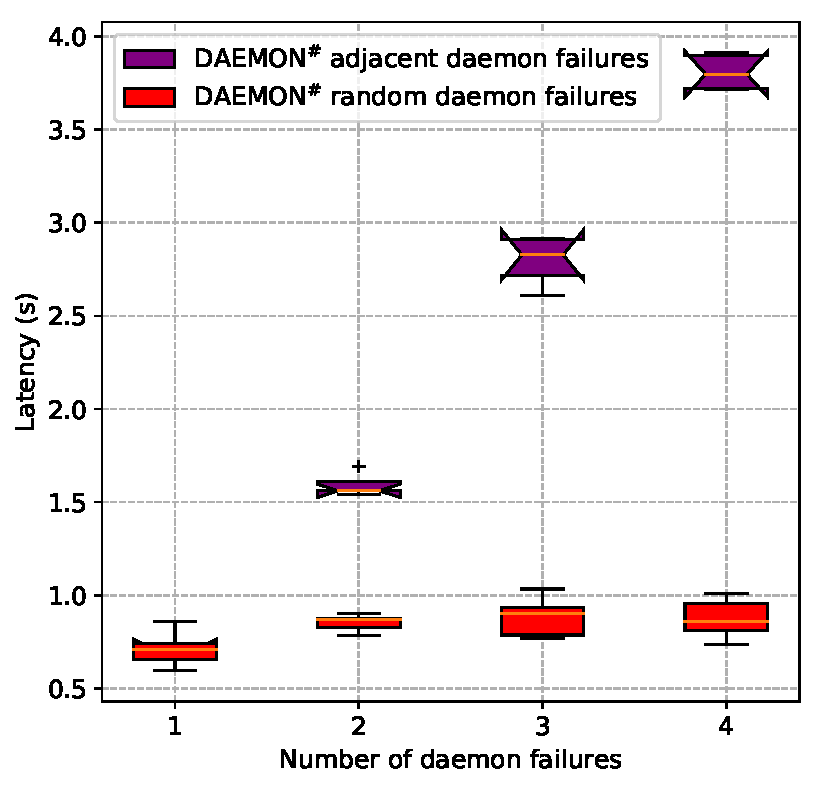
\includegraphics[width=\linewidth]{multi_daemon_failures.pdf}
  \caption{Multiple daemon failures at the same time}
  \label{fig:multi_daemon_failure_nacl}
\end{figure}


\section{Conclusion}\label{sec:conclusion}
Failure detection and propagation is a critical service for resilient systems. In this work, we present an efficient failure detection and propagation design and implementation for distributed systems.
The algorithm is integrated within \prrte so that the detection service
can be employed by a wide variety of clients through a well specified and
popular interface (\pmix). The process and node failure detection strategy presented in this work depends on heartbeats and timeouts. Unlike gossip-based algorithms
it enjoys deterministic communication bounds and overhead to provide a reliable solution that works at scale,
yet it doesn't require an over-specialization detrimental to applicability.
Our design and implementation takes into account of the intricate relationship and trade-offs between system overhead, detection efficiency, and risks: low detection time requires frequent emission of heartbeats messages, increasing the system noise and the risk of false positive. Our solution addresses those concerns and is capable of tolerating high frequency of node and process failures with a low-degree
topology that scales with the number of nodes rather than the number of
managed processes. Our results from different machines and benchmarks
compared to related works shows that \ourwork outperforms non-HPC solutions
significantly, and is competitive with specialized HPC solutions that can
manage only \mpi applications. Thus, this runtime level failure detectors
opens the gate for efficient management of failures for an emerging field
of libraries, programming models, and runtime systems operating on large scale systems.


%\section{Acknowledgments}
%
% The acknowledgments section is defined using the "acks" environment (and NOT an unnumbered section). This ensures
% the proper identification of the section in the article metadata, and the consistent spelling of the heading.
\begin{acks}
%CAARES and ECP OMPIX
This material is based upon work supported by the National Science Foundation under Grant No. (1725692); and the Exascale Computing Project (17-SC-20-SC), a collaborative effort of the
U.S. Department of Energy Office of Science and the National Nuclear Security Administration.
\end{acks}

%
% The next two lines define the bibliography style to be used, and the bibliography file.
\bibliographystyle{ACM-Reference-Format}
\bibliography{sample-base}

\end{document}
%
% If your work has an appendix, this is the place to put it.
\appendix
\end{document}
